\documentclass[aspectratio=169]{beamer}

% Je kan het lettertype iets vergroten door hierboven optie ``14pt'' toe te
% voegen.

%==============================================================================
% Aanloop
%==============================================================================

%---------- Vormgeving --------------------------------------------------------

\usetheme{hogent}

% Kies hieronder een achtergrondkleur
\usecolortheme{hgwhite} % witte achtergrond, zwarte tekst
%\usecolortheme{hgblack} % zwarte achtergrond, witte tekst

%---------- Packages ----------------------------------------------------------

\usepackage[dutch]{babel}      % Nederlandse taal: splitsingen, enz.

\usepackage{booktabs}          % Mooie tabellen
\usepackage{multirow,multicol} % Tabelcellen samenvoegen
\usepackage{eurosym}           % Euro symbool
\usepackage{hyperref}
\hypersetup{
    colorlinks=true,
    linkcolor=blue,
    filecolor=magenta,      
    urlcolor=cyan,
    pdftitle={Overleaf Example},
    pdfpagemode=FullScreen,
}

\urlstyle{same}

%---------- Commando-definities -----------------------------------------------

%---------- Info over de presentatie ------------------------------------------

\title[Korte titel]{Google Scholar zoekresultaten voor wetenschappelijke projecten: linked data \& natural language processing}
\author{Bart De Paepe}
\date{\today}

%==============================================================================
% Inhoud presentatie
%==============================================================================

\begin{document}

%---------- Titelpagina, inhoudstafel -----------------------------------------

\frame{\maketitle}

\begin{frame}
  \frametitle{Inhoud.}

  \tableofcontents
\end{frame}
 
%---------- Corpus ------------------------------------------------------------

\section{Kader.}

\begin{frame}
  \frametitle{Vlaams Instituut voor de Zee}
  \begin{figure}
     
\includegraphics[height=.4\textheight]
      {kader/VLIZ_LOGO.png}
      % Bron: https://www.pexels.com/photo/hand-on-cup-of-coffee-984536/
      
  \end{figure}
  \centering
  \url{https://www.vliz.be}
  
\end{frame}

\begin{frame}
    \frametitle{Integrated Marine Information System}
    \href{https://www.vliz.be/nl/imis}{\begin{figure}
            
\includegraphics[height=.4\textheight]
            {kader/imis.jpg}
            % Bron: https://www.pexels.com/photo/hand-on-cup-of-coffee-984536/
    \end{figure}}
    
    
\end{frame}

\begin{frame}
    \frametitle{Google Scholar}
    \begin{columns}[c]
        % create the column with the first image, that occupies
        % half of the slide
        \begin{column}{.5\textwidth}
            \centering
    \begin{figure}
        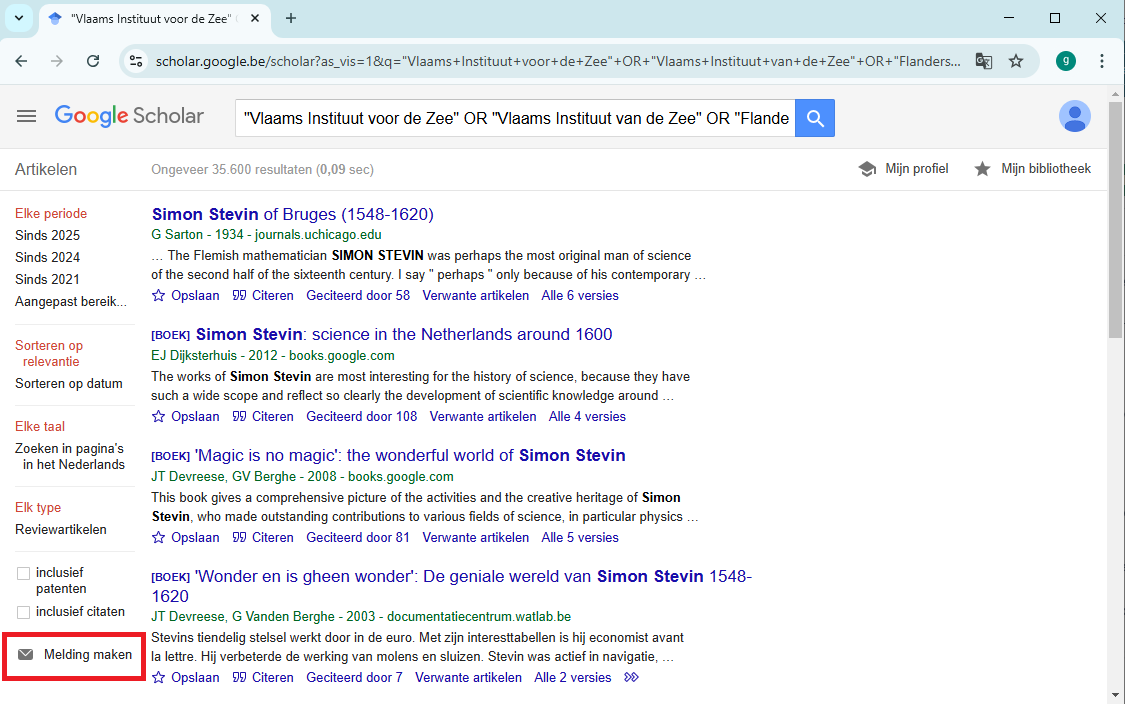
\includegraphics[height=.5\textheight]
        {kader/google-scholar/2_zoekresultaten.PNG}
        % Bron: https://www.pexels.com/photo/hand-on-cup-of-coffee-984536/
        
    \end{figure}
    zoekopdracht
    \end{column}
    \begin{column}{.5\textwidth}
        \centering
    \begin{figure}
        
        
        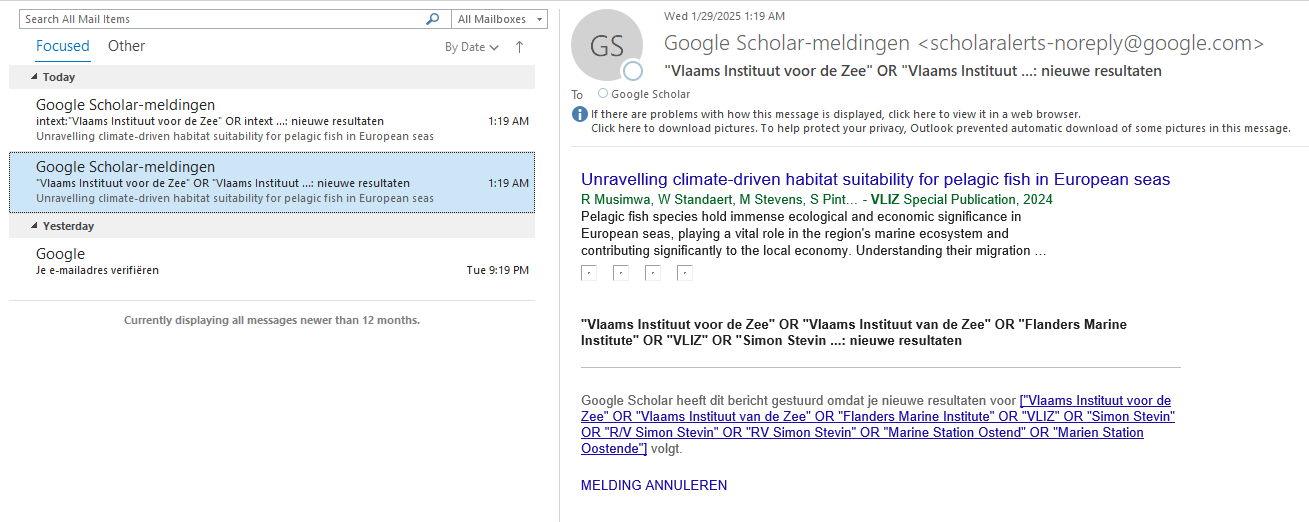
\includegraphics[height=.5\textheight]
        {kader/google-scholar/5_email.PNG}
        % Bron: https://www.pexels.com/photo/hand-on-cup-of-coffee-984536/
        
    \end{figure}
    alert
\end{column}
\end{columns}
    
    
\end{frame}

{
    \setbeamertemplate{background}[pure]%
    {kader/amin-zabardast-Q57aftqNKiE-unsplash.jpg}
\begin{frame}[b]{Title}
    \frametitle{Het probleem.}
    \tiny
    Photo by Amin Zabardast on https://unsplash.com/photos/a-street-sign-on-a-pole-next-to-a-building-Q57aftqNKiE
    
    
\end{frame}
}

\begin{frame}
    \frametitle{De onderzoeksvraag.}
    \small
    ``Hoe kunnen de zoekresultaten van Google Scholar automatisch toegevoegd worden aan IMIS?''
    \begin{itemize}
        \item Hoe kunnen de uiteenlopende zoekresultaten van Google Scholar omgezet worden in gestructureerde data?
        \item Zijn alle zoekresultaten uniek identificeerbaar zodat er geen duplicaten opgeslagen worden?
    \end{itemize}
    \begin{itemize}
        \item Hoe kunnen ook steeds nieuwe zoekresultaten van dezelfde zoekopdracht systematisch opgezocht worden?
        \item Kan er een score berekend worden hoe relevant elk zoekresultaat is ten opzichte van de zoekopdracht?
        \item Als er geen unieke identifier is, hoe wordt er dan gecontroleerd op duplicaten? 
    \end{itemize}
    \begin{itemize}
        \item Hoe blijft de tool overwegend onafhankelijk van third-party software?
        \item Hoe wordt er gegarandeerd dat de tool op de bestaande hardware kan draaien? 
    \end{itemize}
    
    
\end{frame}

\begin{frame}
    \frametitle{Proof of Concept bouwen.}
    Geen grappige afbeelding met auteursrechten hier, wel \href{https://www.slideserve.com/zocha/agile-project-management}{daar}.
    
    
    
\end{frame}

{
    \setbeamertemplate{background}[pure]{methode/arrow.png}
\section{Methode.}
}

\begin{frame}[t]
    \frametitle{Web scraping (1).}
    \begin{columns}[t]
        % create the column with the first image, that occupies
        % half of the slide
        \begin{column}{.5\textwidth}
            \begin{figure}
                
                
                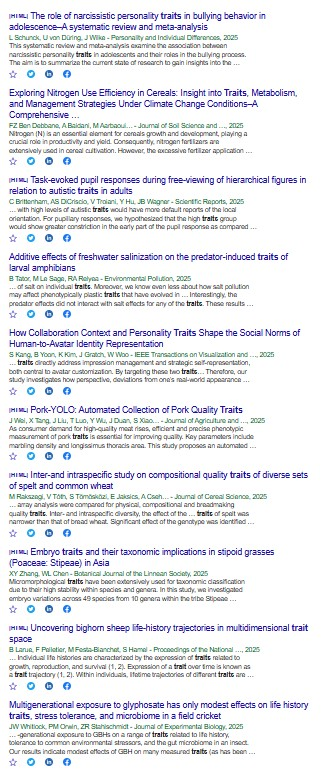
\includegraphics[height=1.5\textheight]
                {methode/web-scraping/SERP.jpg}
                % Bron: https://www.pexels.com/photo/hand-on-cup-of-coffee-984536/
                
            \end{figure}
            
        \end{column}
        \begin{column}{.5\textwidth}
            \begin{figure}
                
                
                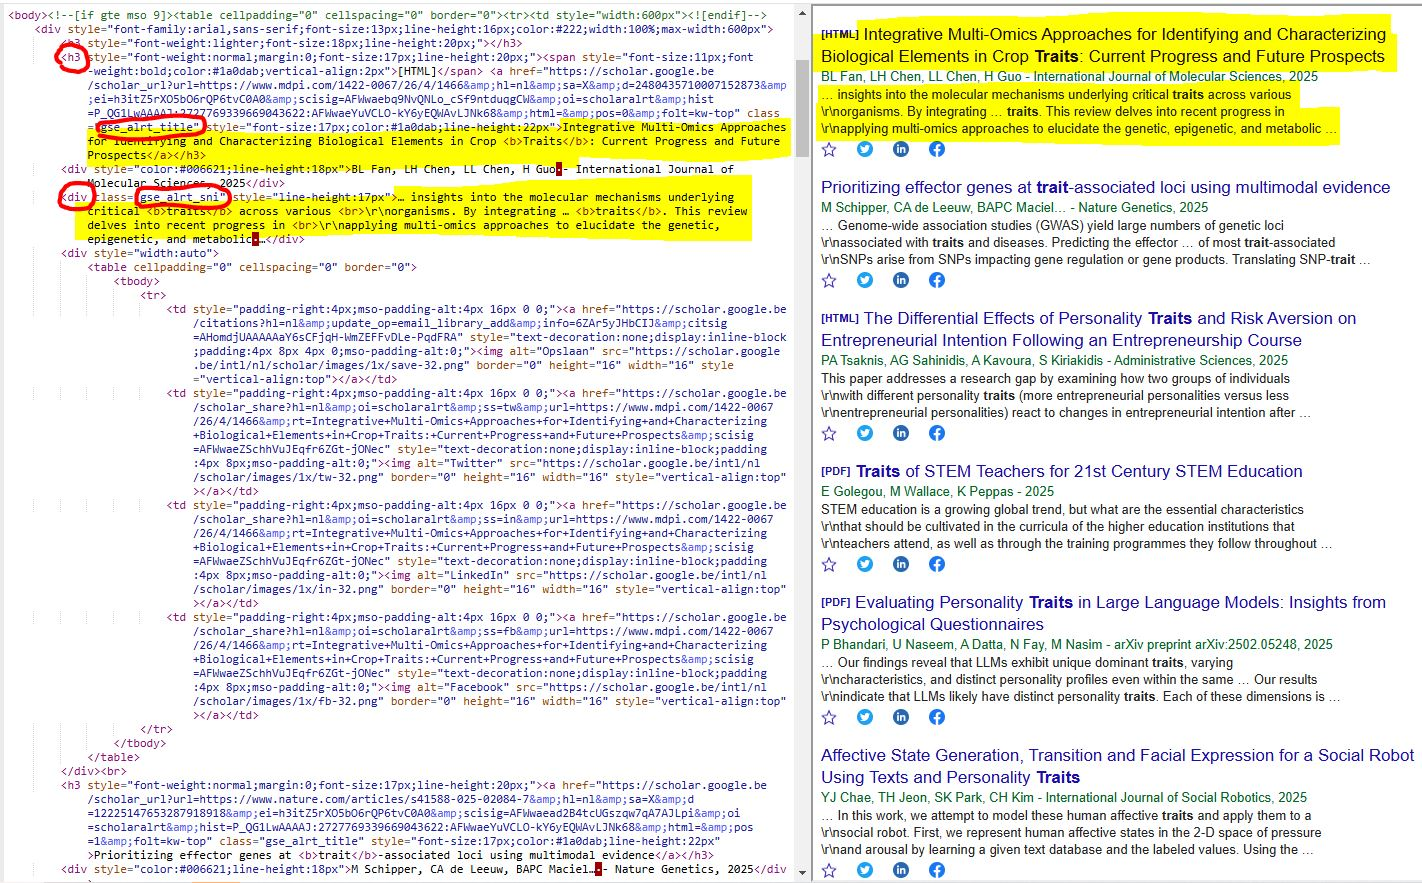
\includegraphics[height=.3\textheight]
                {methode/web-scraping/serp-html.JPG}
                % Bron: https://www.pexels.com/photo/hand-on-cup-of-coffee-984536/
                
            \end{figure}
            
            \begin{listing}
                \begin{lstlisting}
                    \tiny
                    <h3 style="font-weight:normal;margin:0;font-size:17px;line-height:20px;">
                    <span style="fon...lign:2px">[HTML]</span>    
                    <a href="https://www.s...8" \colorbox{hgorange}{class="gse\_alrt\_title"} style="f...t:22px">
                    The role of narcissistic personality <b>traits </b>in bullying behavior 
                    in adolescence–A systematic review and meta-analysis
                    </a>
                    </h3>
                \end{lstlisting}
                
            \end{listing}
        \end{column}
    \end{columns}
\end{frame}

\begin{frame}
    \frametitle{Web scraping (2).}
    \begin{columns}[c]
        % create the column with the first image, that occupies
        % half of the slide
        \begin{column}{.5\textwidth}
    \begin{itemize}
        \item \href{https://github.com/bart-de-paepe/google-scholar-openai/blob/main/app/src/services/parse_service.py}{OpenAI (AKA ChatGPT)}
    
    \item \href{https://github.com/bart-de-paepe/google-scholar-beautifulsoup/blob/main/app/src/services/parse_service.py}{Beautiful Soup}
\end{itemize}
\end{column}
\begin{column}{.5\textwidth}
    \begin{figure}
        
        
        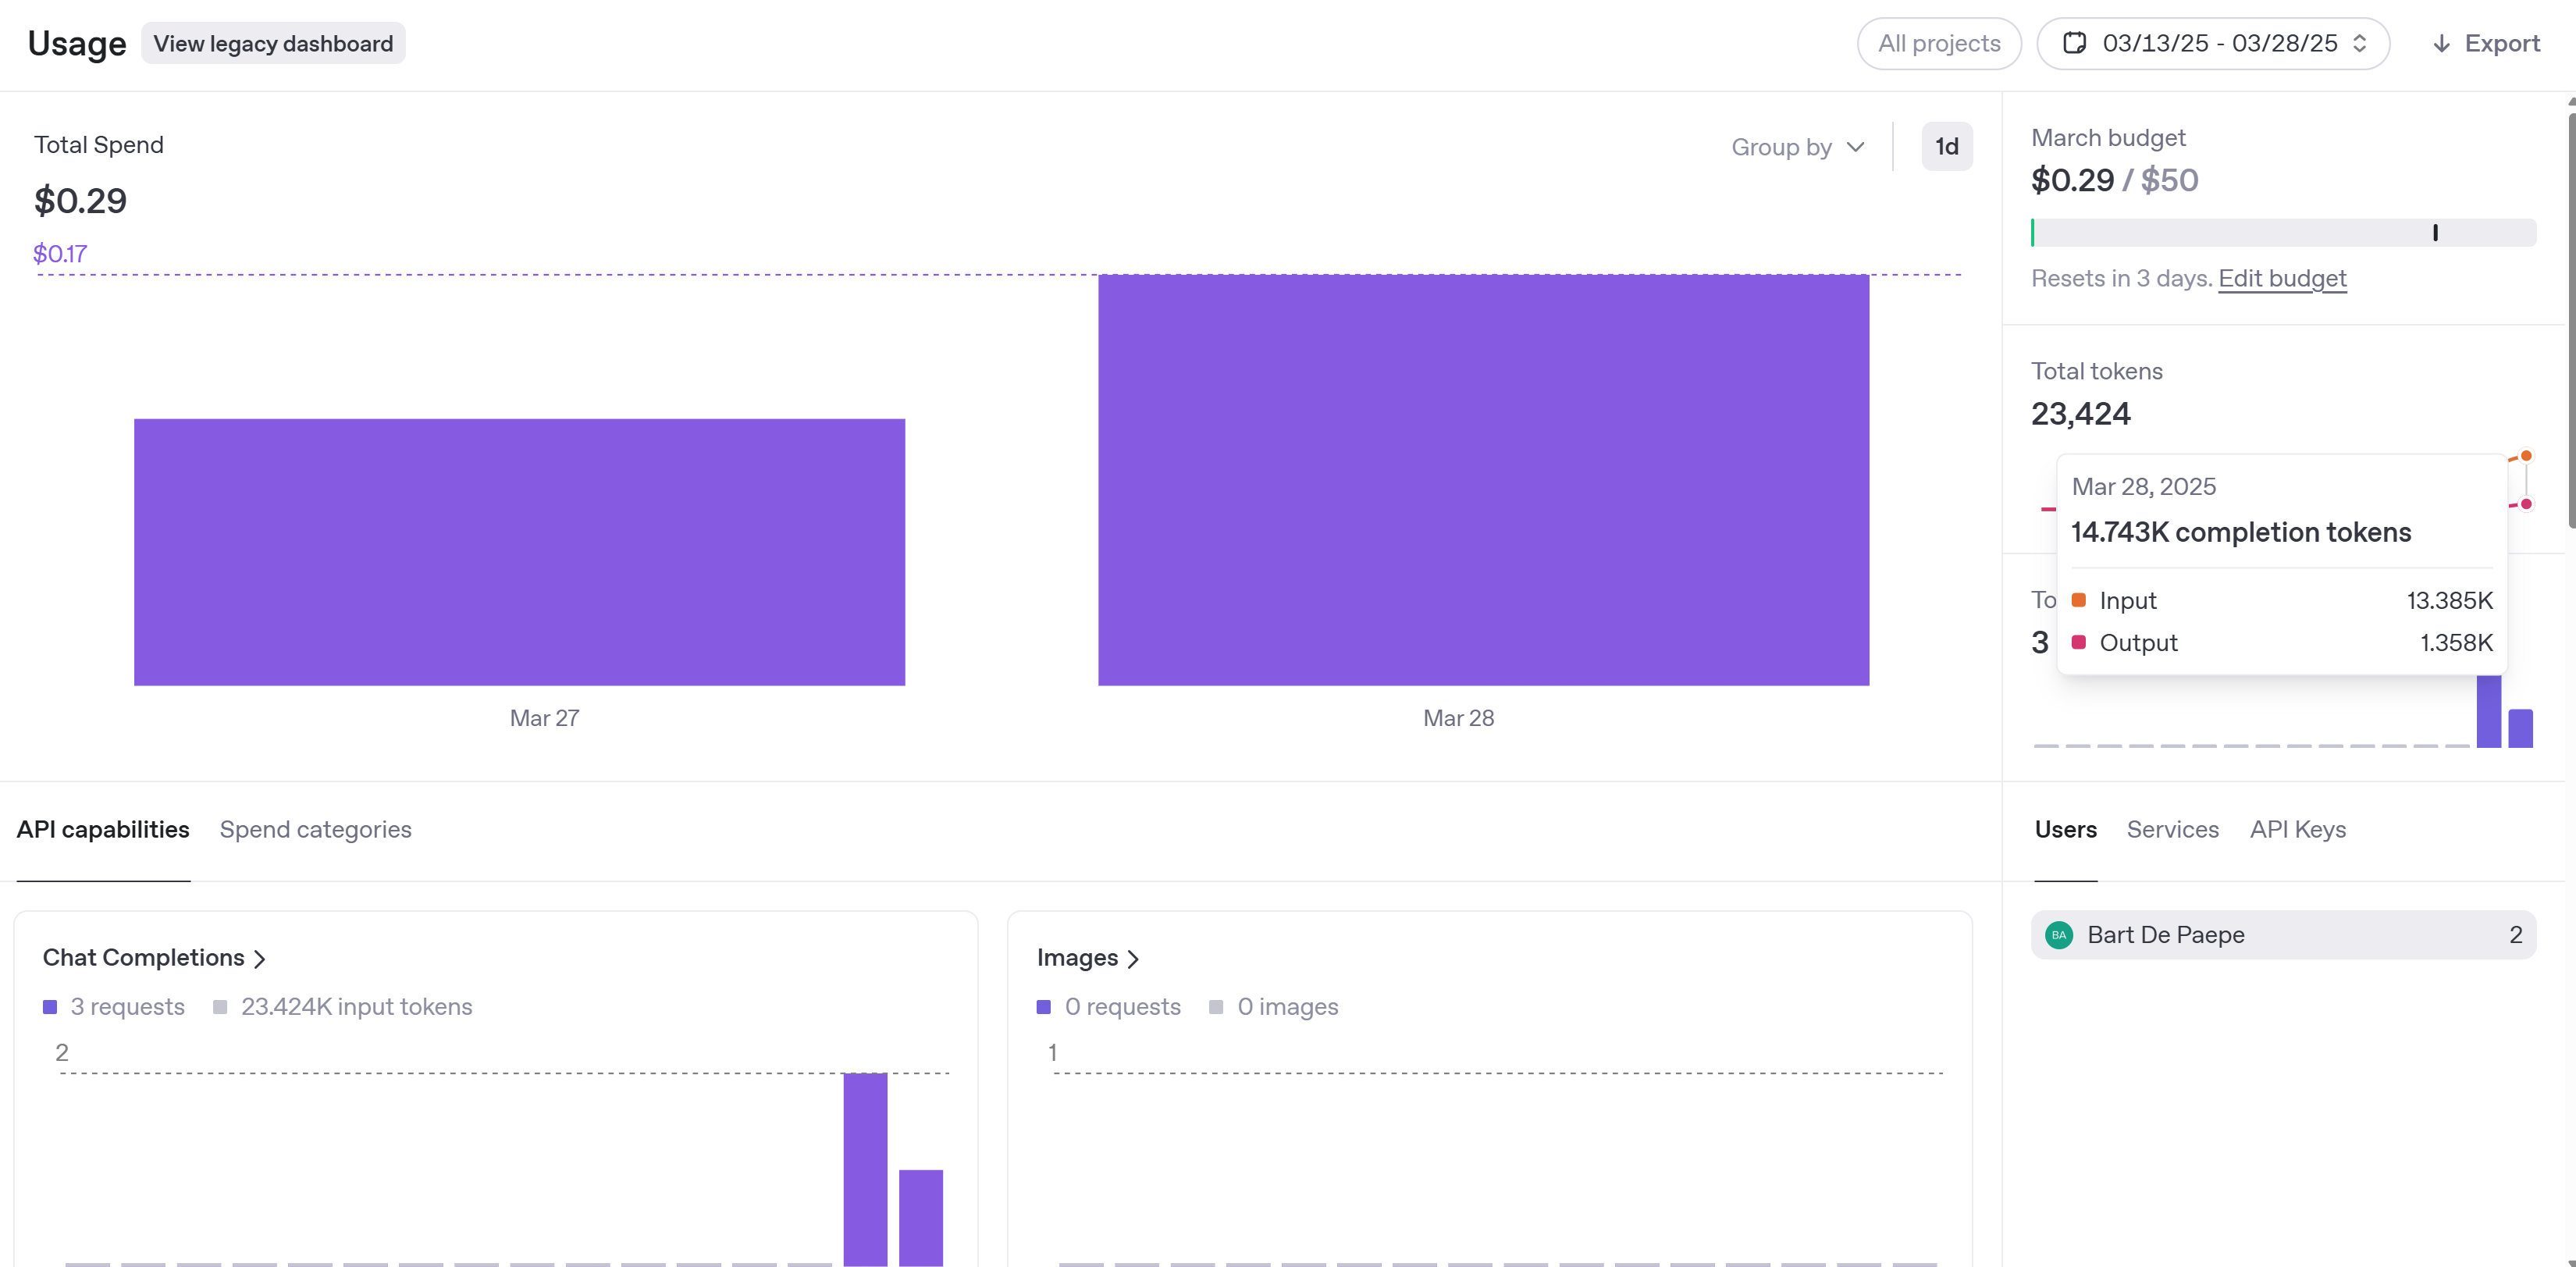
\includegraphics[height=.5\textheight]
        {methode/web-scraping/openai_billing.png}
        % Bron: https://www.pexels.com/photo/hand-on-cup-of-coffee-984536/
        
    \end{figure}
\end{column}
\end{columns}
\end{frame}

\begin{frame}
\frametitle{Natural language processing.}
\begin{itemize}
    \item "Anna vertelde dat ze morgen naar de universiteit gaat omdat ze daar een belangrijk examen heeft."
    \item "Anna vertelde dat Anna morgen naar de universiteit gaat omdat Anna daar een belangrijk examen heeft."
    \item "Anna vertelde morgen universiteit gaat Anna belangrijk examen"
    \item "Anna vertel morgen universiteit gaan Anna belangrijk examen"
\end{itemize}


\end{frame}

\begin{frame}
\frametitle{Linked data (1).}
\begin{columns}[c]
    % create the column with the first image, that occupies
    % half of the slide
    \begin{column}{.5\textwidth}
        \centering
        \begin{figure}
            
            
            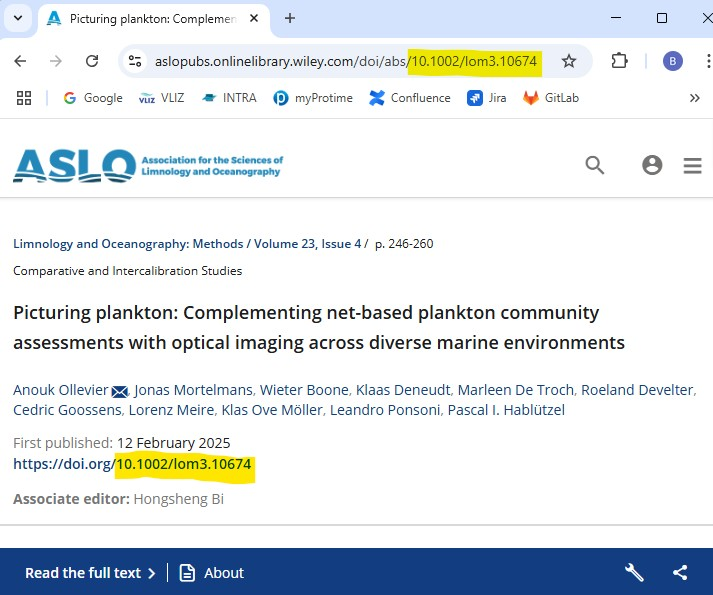
\includegraphics[height=.5\textheight]
            {methode/linked-data/DOI_Link.jpg}
            % Bron: https://www.pexels.com/photo/hand-on-cup-of-coffee-984536/
            
        \end{figure}
        DOI in de URL \& op de webpagina
        
\end{column}
\begin{column}{.5\textwidth}
    \centering
    \begin{figure}
        
        
        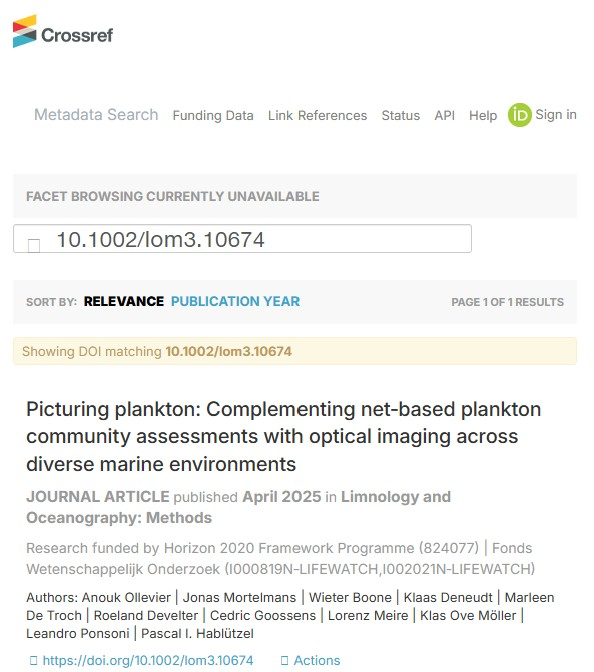
\includegraphics[height=.5\textheight]
        {methode/linked-data/DOI_Crossref.jpg}
        % Bron: https://www.pexels.com/photo/hand-on-cup-of-coffee-984536/
        
    \end{figure}
    DOI in Crossref
\end{column}
\end{columns}
\end{frame}

\begin{frame}
\frametitle{Linked data (2).}
\begin{columns}[c]
    % create the column with the first image, that occupies
    % half of the slide
    \begin{column}{.5\textwidth}
        \centering
        \begin{figure}
            
            
            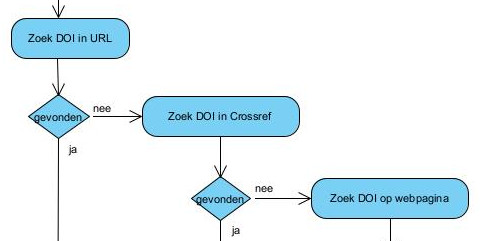
\includegraphics[height=.5\textheight]
            {methode/linked-data/DOI_flow.jpg}
            % Bron: https://www.pexels.com/photo/hand-on-cup-of-coffee-984536/
            
        \end{figure}
        flowchart om de DOI op te zoeken
    \end{column}
    \begin{column}{.5\textwidth}
        \centering
        verschillende types webpagina's
        \begin{itemize}
            \item een gewone HTML pagina
            \item een PDF document
            \item een webpagina met een embedded PDF document
        \end{itemize}
    \end{column}
\end{columns}
\end{frame}

\begin{frame}[t]{Title}
\frametitle{Semantic search (1).}
\begin{minipage}[t][0.8715\textheight]{\textwidth}
    \begin{columns}[c]
        % create the column with the first image, that occupies
        % half of the slide
        \begin{column}{.5\textwidth}
            \centering
            Google Scholar zoekresultaat
            \begin{figure}
                
                
                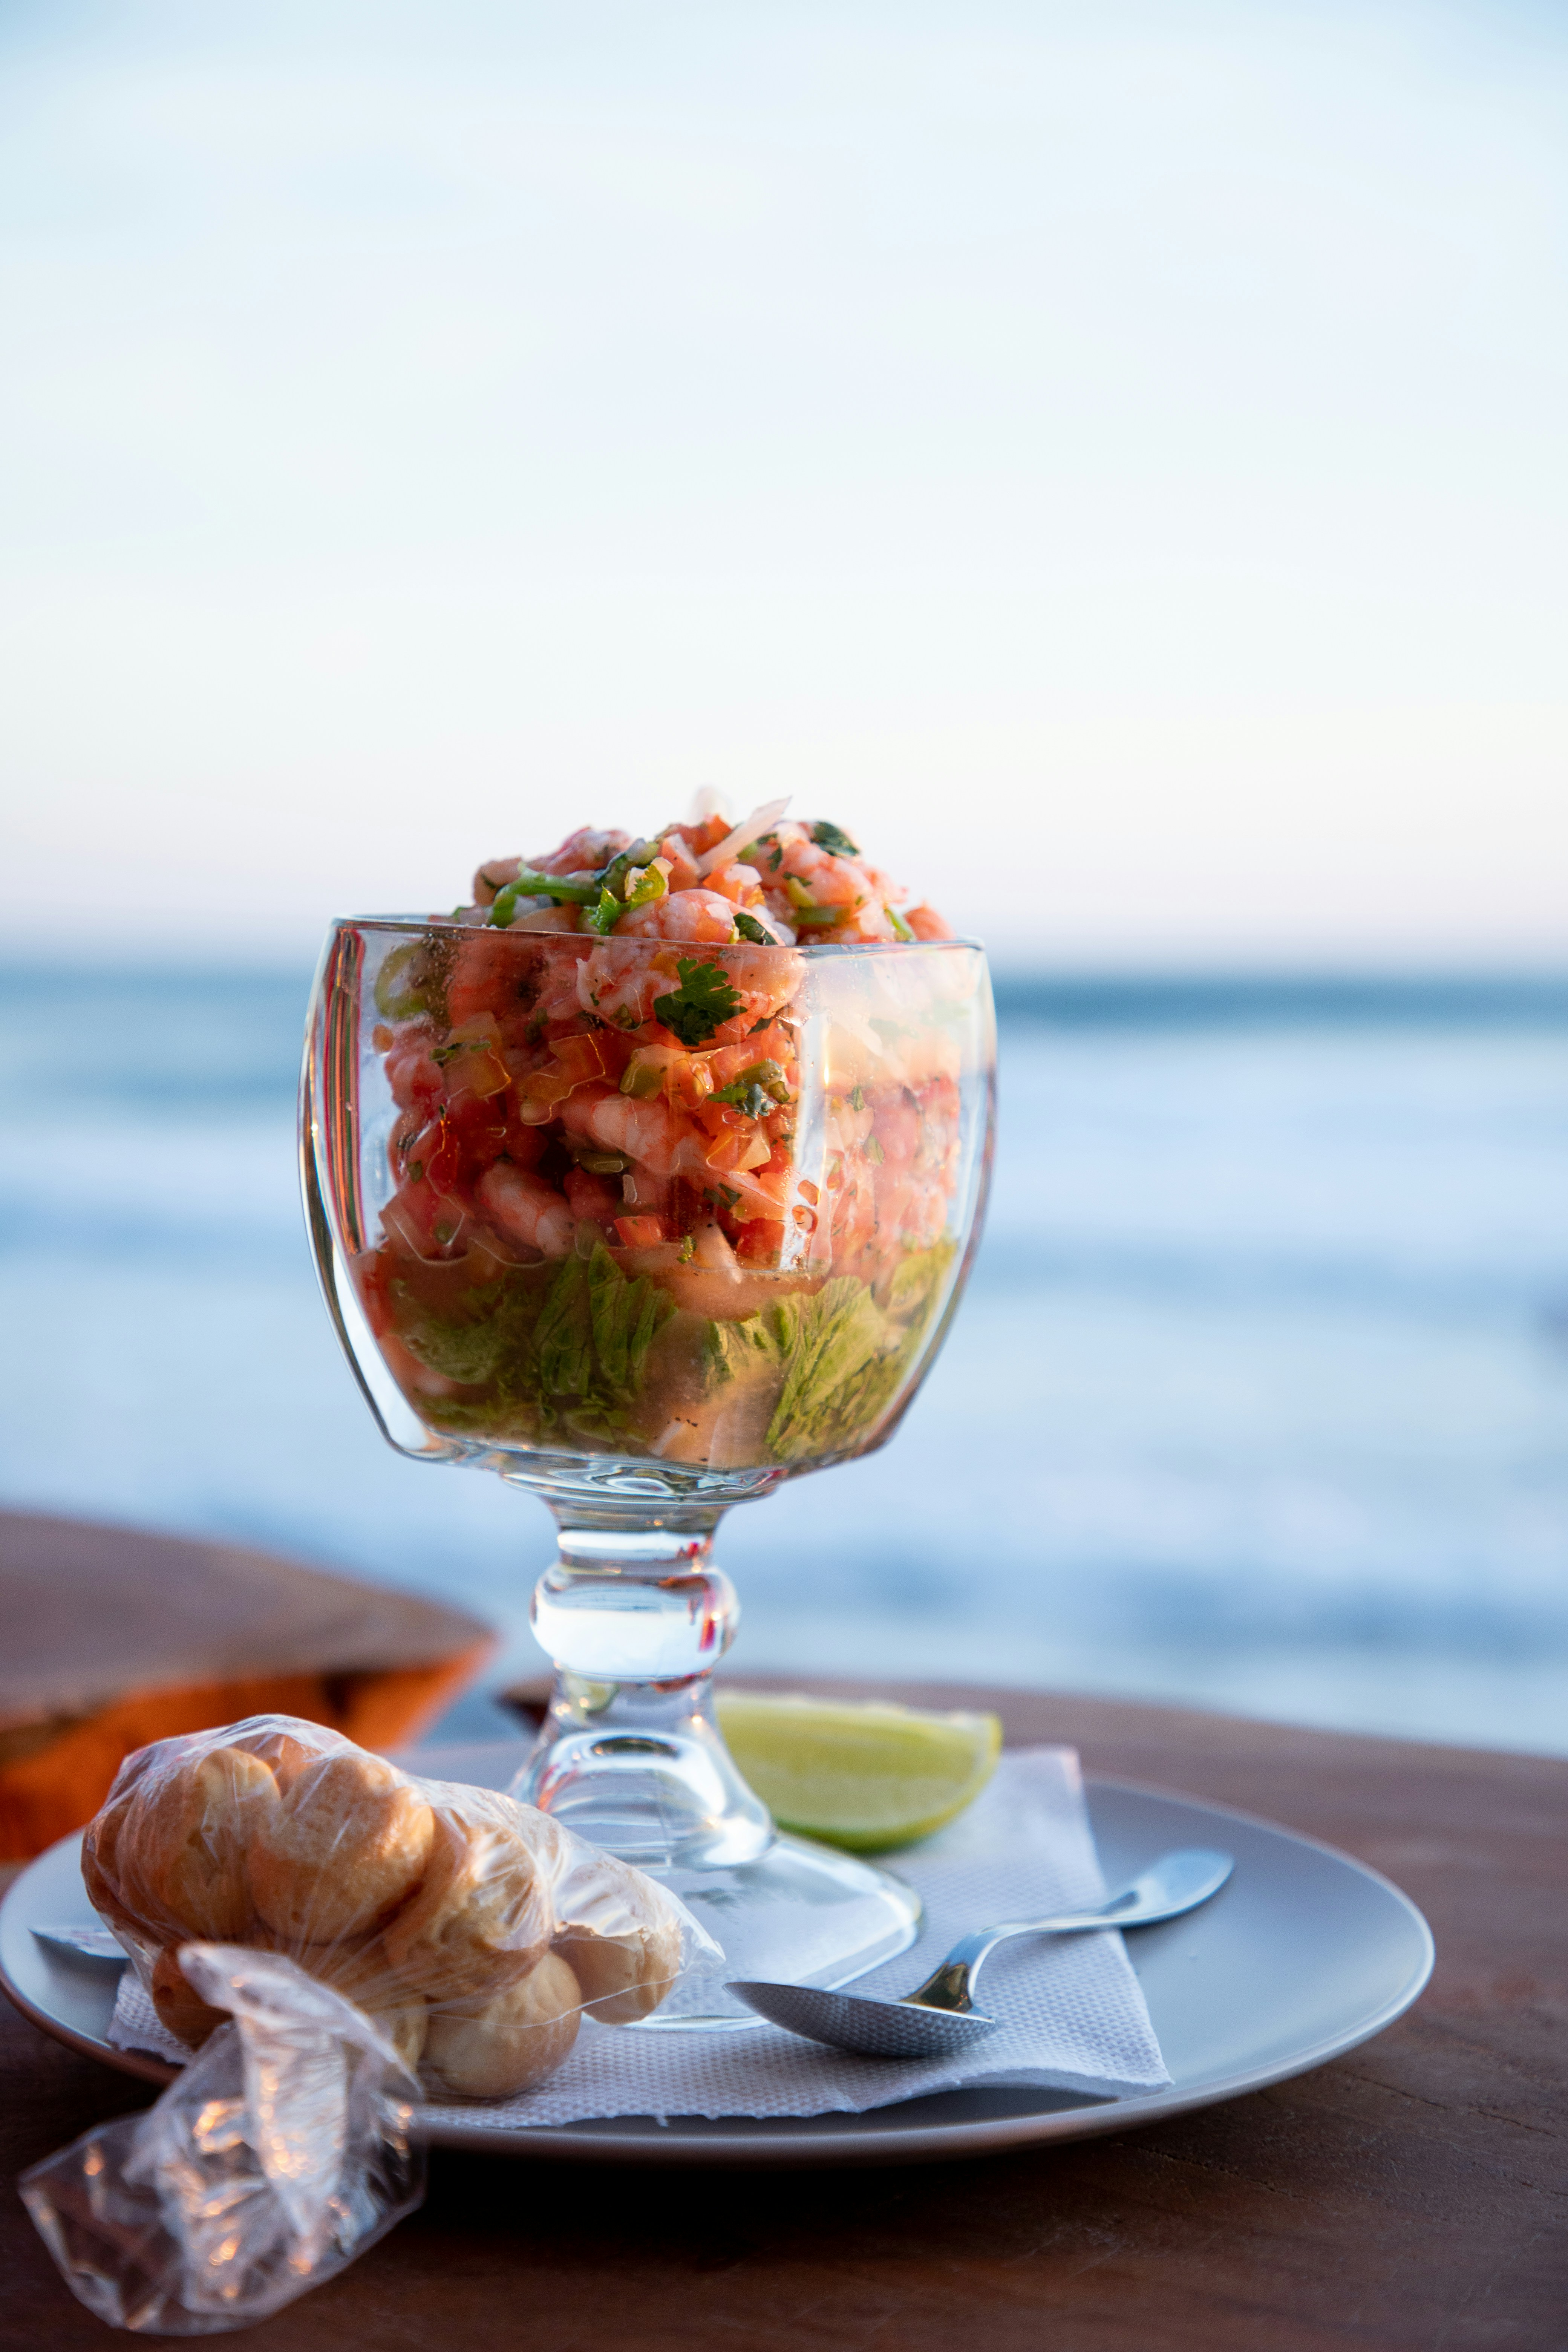
\includegraphics[height=.5\textheight]
                {methode/semantic-search/schrimp.jpg}
                % Bron: https://www.pexels.com/photo/hand-on-cup-of-coffee-984536/
                
            \end{figure}
            
            
            
        \end{column}
        \begin{column}{.5\textwidth}
            \centering
            publicatie in IMIS
            \begin{figure}
                
                
                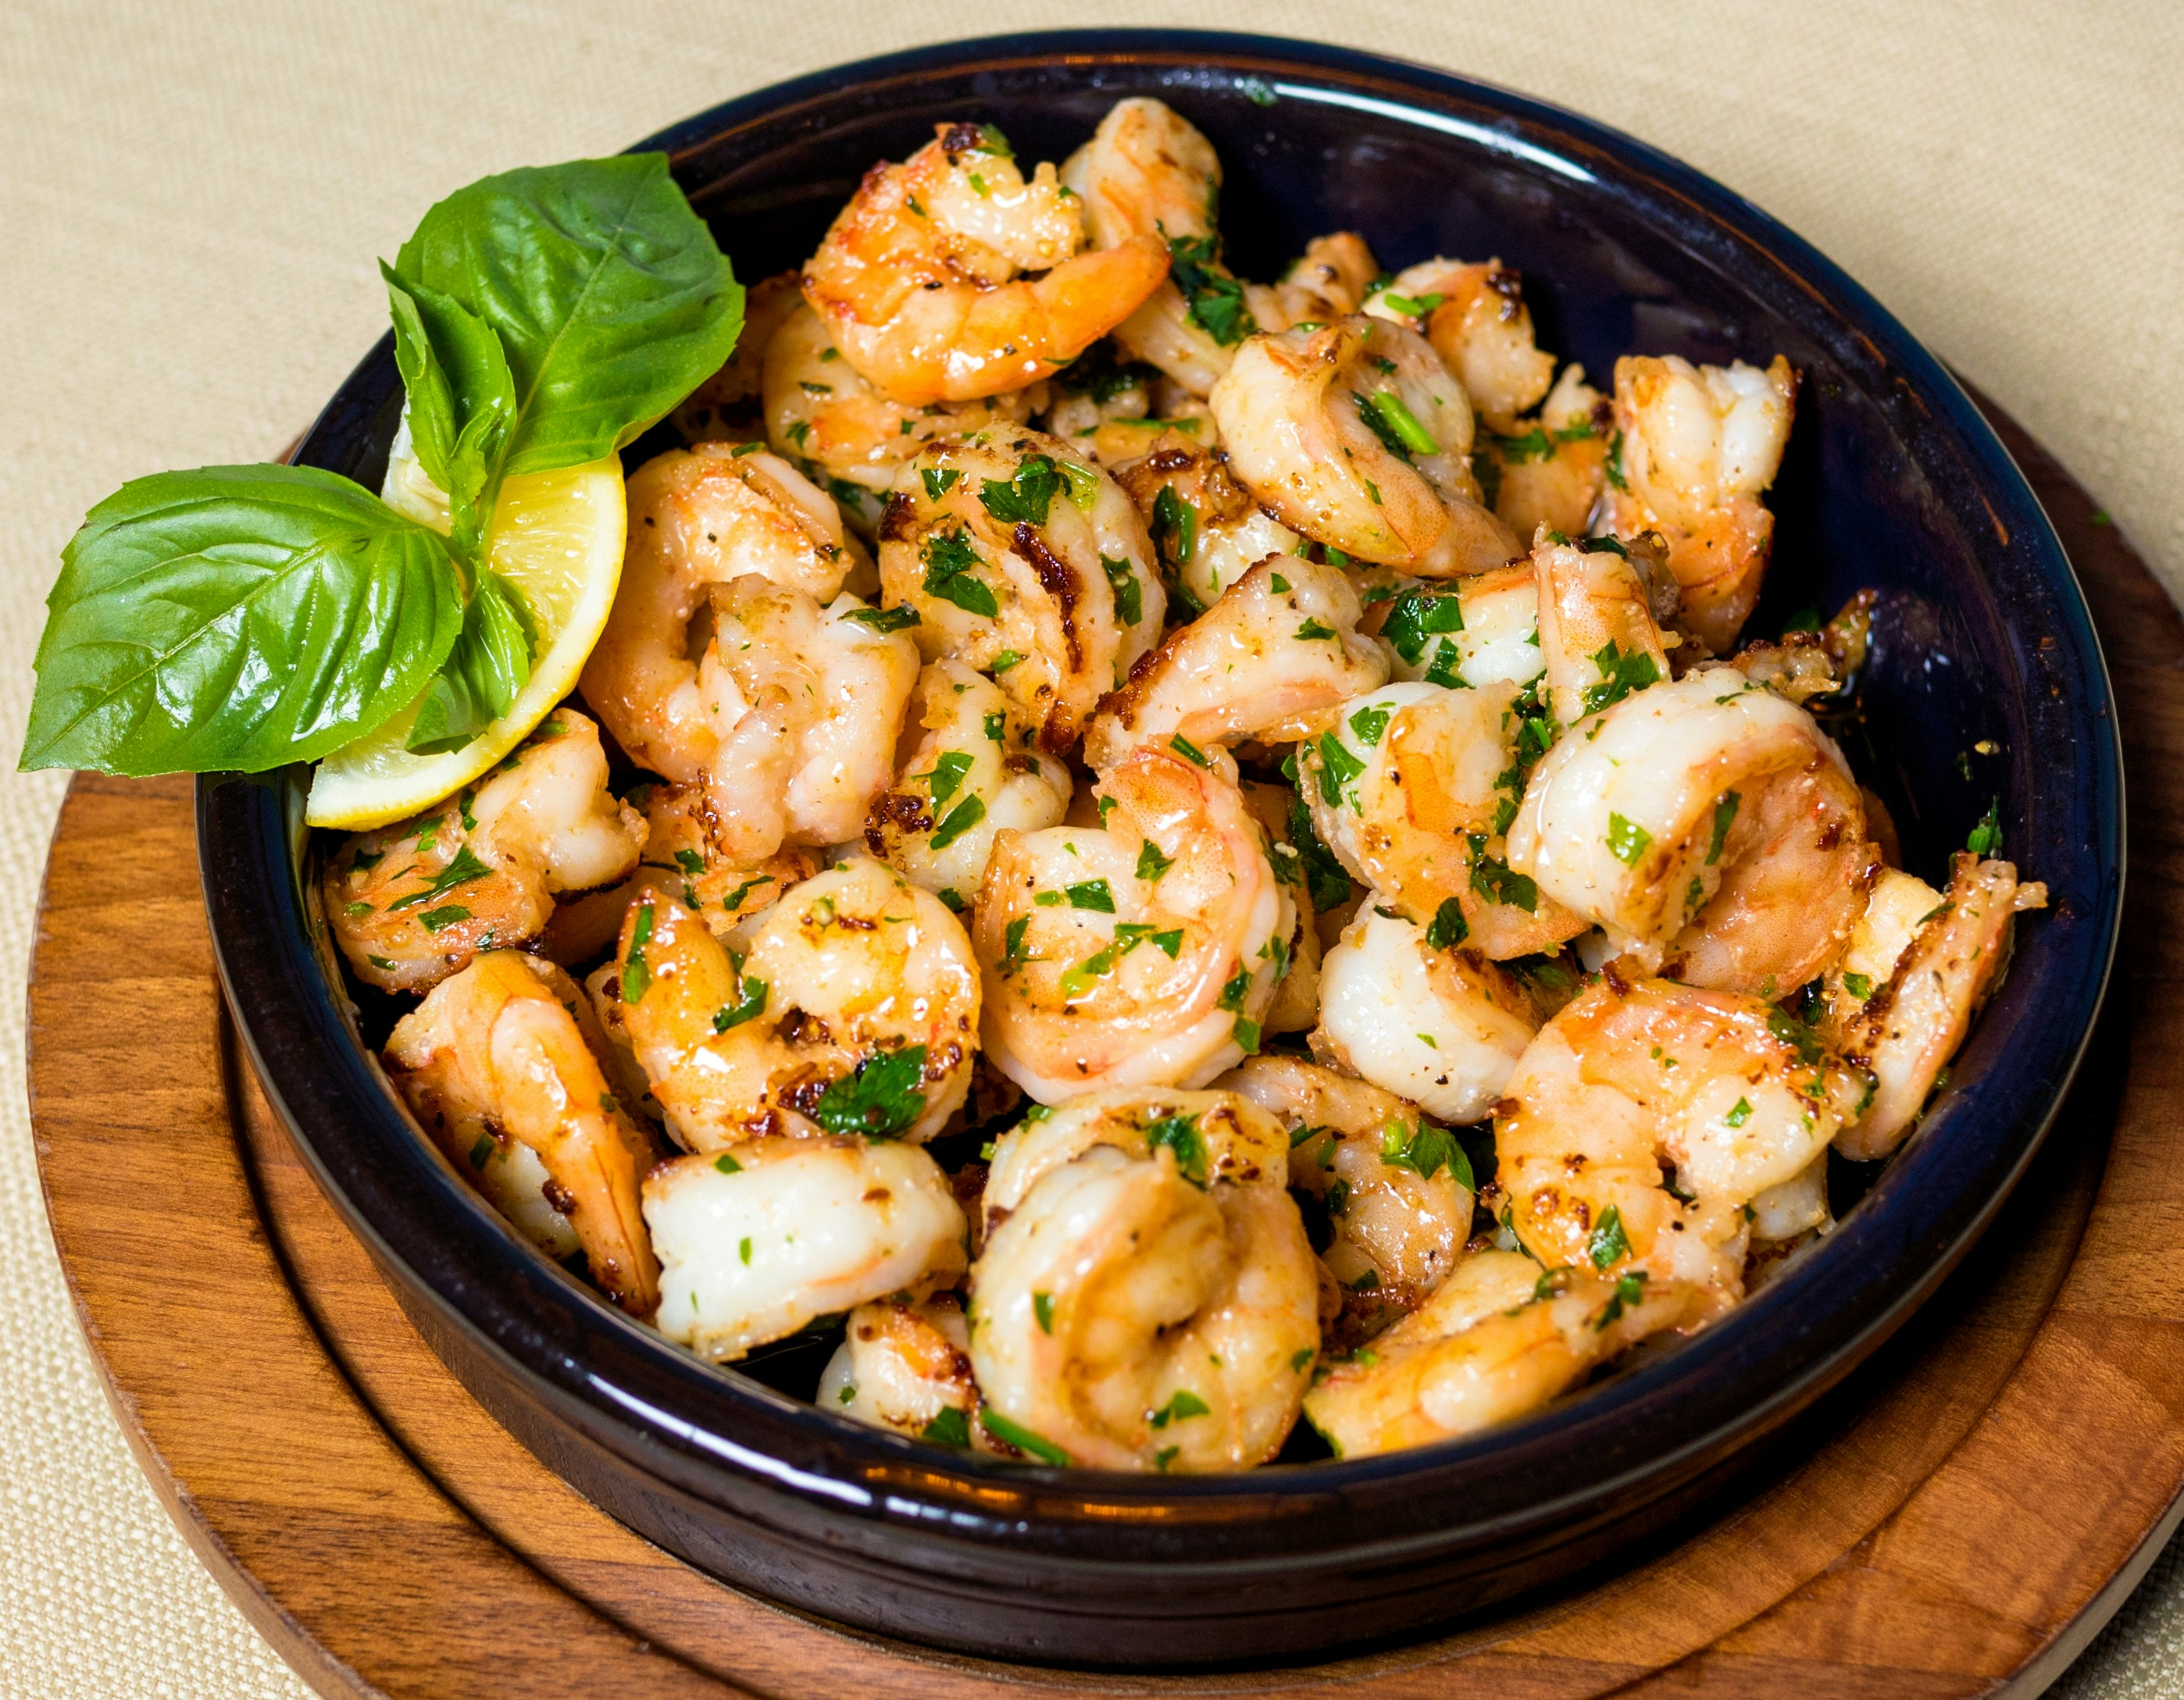
\includegraphics[height=.5\textheight]
                {methode/semantic-search/prawn.jpg}
                % Bron: https://www.pexels.com/photo/hand-on-cup-of-coffee-984536/
                
            \end{figure}
        \end{column}
    \end{columns}
    \url{https://www.youtube.com/watch?v=QSW2L8dkaZk}
    
    \vspace{\fill}% or \vfill
    \tiny
    Photo by Yasmine Duchesne on https://unsplash.com/photos/clear-footed-glass-with-red-and-yellow-liquid-on-table-VSb6KDaiga0
    Photo by Farhad Ibrahimzade on https://unsplash.com/photos/cooked-food-on-black-ceramic-bowl-HNmcgpzPHag
    
    
\end{minipage}

\end{frame}

\begin{frame}
\frametitle{Semantic search (2).}
\begin{columns}[c]
    % create the column with the first image, that occupies
    % half of the slide
    \begin{column}{.5\textwidth}
        
                \begin{figure}
                    \caption{embeddings}
                    
                    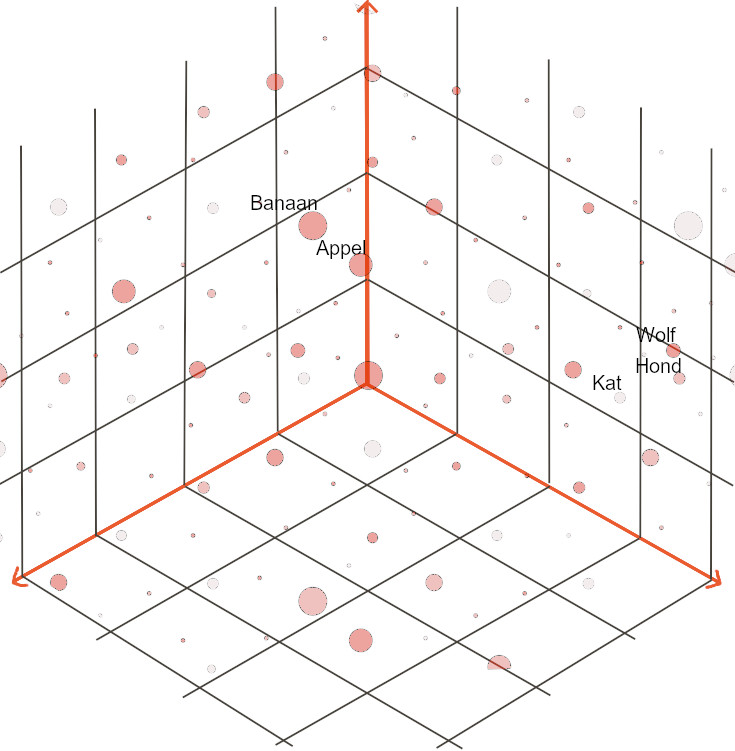
\includegraphics[height=.5\textheight]
                    {methode/semantic-search/word2vec2.jpg}
                    % Bron: https://www.pexels.com/photo/hand-on-cup-of-coffee-984536/
                    \label{img:voorbeeld}
                \end{figure}
            
    \end{column}
    \begin{column}{.5\textwidth}
        \begin{figure}
            \caption{schema}
            
            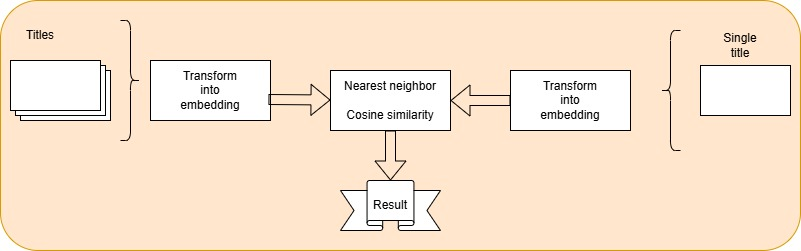
\includegraphics[height=.5\textheight]
            {methode/semantic-search/embeddings.jpg}
            % Bron: https://www.pexels.com/photo/hand-on-cup-of-coffee-984536/
            \label{img:voorbeeld}
        \end{figure}
    \end{column}
\end{columns}
\end{frame}

\begin{frame}
    \frametitle{Proof of Concept}
    \begin{figure}
        \caption{activity diagram}
        
        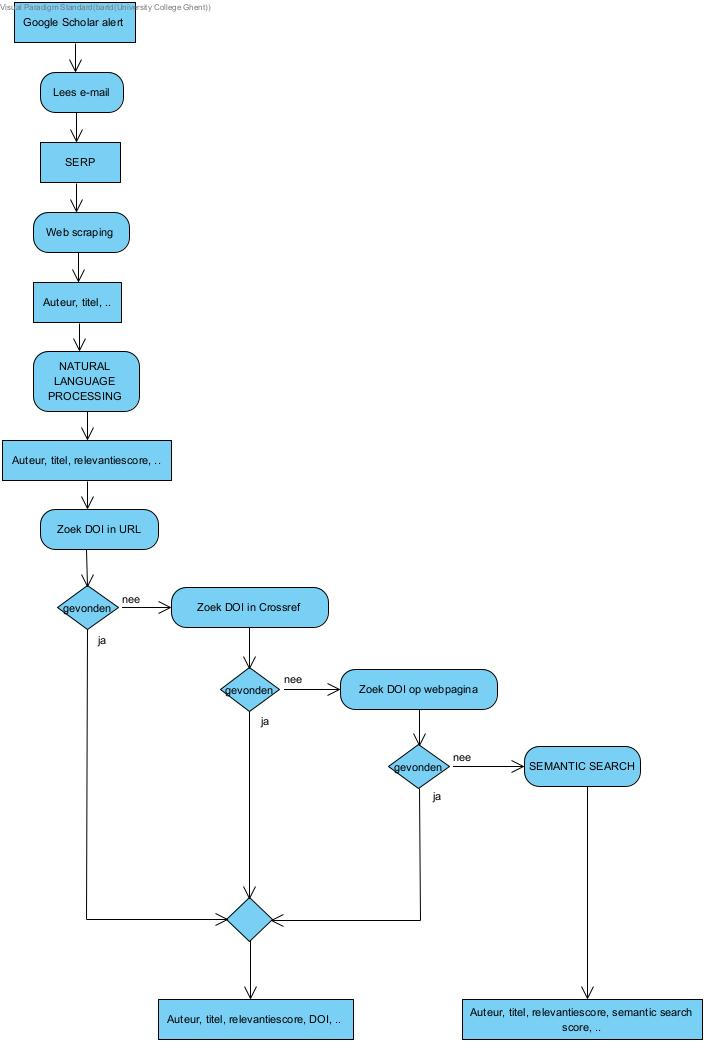
\includegraphics[height=.4\textheight]
        {methode/activity-diagram.jpg}
        % Bron: https://www.pexels.com/photo/hand-on-cup-of-coffee-984536/
        \label{img:voorbeeld}
    \end{figure}
    
\end{frame}

\section{Resultaten.}


\begin{frame}
    \frametitle{Resultaten (1).}
    \begin{columns}[c]
        % create the column with the first image, that occupies
        % half of the slide
        \begin{column}{.5\textwidth}
            \begin{figure}
                \caption{Zoekresultaten voor VLIZ}
                
                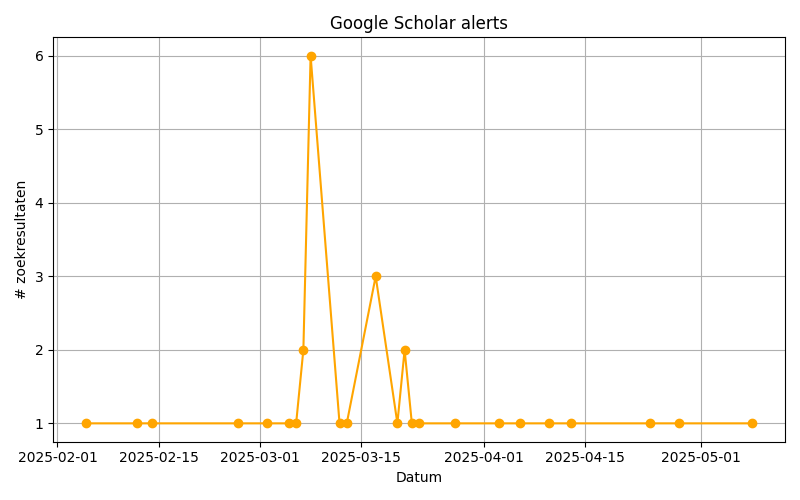
\includegraphics[height=.5\textheight]
                {resultaten/GS_alerts_timeline.png}
                % Bron: https://www.pexels.com/photo/hand-on-cup-of-coffee-984536/
                \label{img:voorbeeld}
            \end{figure}
        \end{column}
        \begin{column}{.5\textwidth}
            \begin{itemize}
                \item 23 alerts
                \item 1-6 zoekresultaten per alert
                \item 48\% van de zoekresultaten DOI
            \end{itemize}
        \end{column}
    \end{columns}
    
\end{frame}

\begin{frame}
\frametitle{Resultaten (2).}
\begin{columns}[c]
    % create the column with the first image, that occupies
    % half of the slide
    \begin{column}{.5\textwidth}
        \begin{figure}
            \caption{Use cases}
            
            
\includegraphics[height=.5\textheight]
            {resultaten/GS_alerts_auteurtijdschriftjaartal.jpg}
            % Bron: https://www.pexels.com/photo/hand-on-cup-of-coffee-984536/
            \label{img:voorbeeld}
        \end{figure}
    \end{column}
    \begin{column}{.5\textwidth}
        \begin{table}[h!]
            \tiny
            \caption{e-mail 25-04-24}
            \centering
            \begin{tabularx}{\textwidth}{|p{4cm}|X|} 
                \hline
                \multicolumn{2}{|X|}{\textbf{zoekresultaat}} \\
                \hline
                web &\textbf{titel}: VLIZ Jaarverslag voor Schenkers 2024\\
                scraping&\textbf{link}: https://www.vliz.be/projects/trophos/\\&imis.php?module\textbackslash x3dref\textbackslash x26refid\textbackslash x3d406498\\
                &\textbf{auteur}: VLIZ\\
                &\textbf{tijdschrift}: -\\
                &\textbf{jaar}: -\\
                &\textbf{tekst}: Zee als Goed Doel ontving in 2024 als eerste wereldwijd de erkenning als Grant Making Facility ter ondersteuning van het Decennium van Oceaanwetenschappen voor Duurzame Ontwikkeling (2021-2030). Dit stelt De Zee als Goed Doel in staat …\\
                \hline
                NLP&\textbf{relevantiescore}: 0.250753012935632\\
                \hline
                DOI&\textbf{DOI}: -\\
                &\textbf{bron}: -\\
                \hline
                semantic&\textbf{semantic search score}: 0.8377995491027832\\
                search&\\
                \hline
            \end{tabularx}
            \label{table:email20250424}
        \end{table}
    \end{column}
\end{columns}

\end{frame}

\section{Discussie.}

\begin{frame}
\frametitle{Discussie.}
\begin{itemize}
    \item Het automatisch opzoeken van de DOI is de grootste meerwaarde van de tool.
    \item Gebruikers kunnen focussen op publicaties zonder DOI en/of met een lage relevantiescore.
    \item 1500-200 publicaties per jaar: 5-6 VTE
    \item Met de tool potentiële verlaging tot 2-3 VTE
    \end{itemize}


\end{frame}

\section{Conclusie.}

\begin{frame}
\frametitle{Conclusie.}
\begin{itemize}
    \item Tool zal gebruikt worden binnen het VLIZ.
    \item Korte termijn: Verbeteringen door meer gelinkte data (auteurs, tijdschriften) op te zoeken in IMIS.
    \item Lange termijn: Uitvoerige tests met LLMs (is niet onderhevig aande structuur van de HTML)
\end{itemize}

\end{frame}

\begin{frame}
    \frametitle{Woord van dank.}
    \begin{itemize}
        \item Bart Vanhoorne
        \item Milan Lamote
        \item Jan Claes
        \item Fons Verheyde
        \item Cedric Decruw
        \item Lies Knockaert
    \end{itemize}
    
\end{frame}

\end{document}
